\documentclass[12pt,a4paper]{article}

\usepackage[utf8]{inputenc}
\usepackage[spanish]{babel}
\usepackage{geometry}
\usepackage{graphicx}
\usepackage{float}
\usepackage{booktabs}
\usepackage{array}
\usepackage{listings}
\usepackage{xcolor}
\usepackage{tikz}
\usepackage{hyperref}

\geometry{margin=2.5cm}

\lstset{
    basicstyle=\ttfamily\small,
    breaklines=true,
    frame=single,
    numbers=left,
    numberstyle=\tiny,
    keywordstyle=\bfseries,
    commentstyle=\itshape,
    showstringspaces=false
}

\title{\textbf{Informe de Práctica: Diseño y Fragmentación de una Base de Datos Distribuida}}
\author{
Estudiante: Freddy Vladimir\\
Universidad Técnica Estatal de Quevedo\\
Facultad de Ciencias de la Computación\\
Carrera de Ingeniería de Software\\
Asignatura: Aplicaciones Distribuidas ISR-701
}
\date{Período Regular 2026--2027}

\begin{document}

\maketitle

\section{Introducción}

La presente práctica tiene como finalidad diseñar e implementar una base de datos distribuida mediante técnicas de fragmentación horizontal, vertical y mixta. Para ello se utilizó PostgreSQL 16 dentro de contenedores Docker, simulando tres nodos independientes que representan las sedes Campus, Babahoyo y Ventanas.

La fragmentación de bases de datos permite dividir la información en partes más pequeñas, llamadas fragmentos, que pueden almacenarse en diferentes nodos. Esta estrategia mejora la organización de los datos, permite acercar la información al lugar donde más se utiliza y facilita el crecimiento de un sistema distribuido \cite{amer2020ddbs, ge2021knosys}. En esta práctica se trabajó con el escenario de una cafetería universitaria que registra clientes, productos y pedidos.

El objetivo principal fue comprobar que una base de datos puede ser dividida físicamente en varios nodos y, posteriormente, reconstruida mediante vistas globales usando \texttt{postgres\_fdw}. Además, se verificaron las tres condiciones fundamentales de una fragmentación correcta: completitud, reconstrucción y disjunción.

\section{Entorno de trabajo}

Para el desarrollo de la práctica se utilizó un entorno local basado en Docker Desktop, PostgreSQL 16 y PowerShell. El proyecto fue gestionado desde IntelliJ IDEA, donde se organizaron los archivos SQL, el archivo \texttt{docker-compose.yml}, el archivo \texttt{README.md} y el informe en \LaTeX.

La estructura principal del proyecto fue la siguiente:

\begin{lstlisting}
practica-fragmentacion/
|
|-- docker-compose.yml
|-- README.md
|-- sql/
|   |-- 01_esquema_central.sql
|   |-- 02_datos.sql
|   |-- 03_fragmentacion_horizontal.sql
|   |-- 04_fragmentacion_vertical.sql
|   |-- 05_fragmentacion_mixta.sql
|   |-- 06_vistas_globales.sql
|   |-- 07_verificacion.sql
|
|-- informe/
    |-- informe.tex
    |-- capturas/
\end{lstlisting}

Se levantaron tres contenedores PostgreSQL. Cada contenedor representa un nodo de la base de datos distribuida.

\begin{table}[H]
\centering
\caption{Nodos utilizados en la práctica}
\begin{tabular}{llll}
\toprule
\textbf{Nodo} & \textbf{Contenedor} & \textbf{Puerto local} & \textbf{Base de datos} \\
\midrule
Campus & pg-campus & 5433 & cafeteria \\
Babahoyo & pg-babahoyo & 5434 & cafeteria \\
Ventanas & pg-ventanas & 5435 & cafeteria \\
\bottomrule
\end{tabular}
\end{table}

Los tres contenedores fueron levantados con el comando:

\begin{lstlisting}
docker compose up -d
\end{lstlisting}

Posteriormente se verificó su estado con:

\begin{lstlisting}
docker compose ps
\end{lstlisting}

\section{Modelo de datos centralizado}

Antes de realizar la fragmentación, se creó un esquema centralizado en el nodo \texttt{pg-campus}. Este esquema sirvió como referencia para comparar los resultados después de dividir los datos.

El modelo utilizado contiene tres tablas principales: \texttt{clientes}, \texttt{productos} y \texttt{pedidos}. La tabla \texttt{clientes} almacena la información de los usuarios de la cafetería, la tabla \texttt{productos} contiene los productos disponibles y la tabla \texttt{pedidos} registra las ventas realizadas.

\begin{figure}[H]
\centering
\begin{tikzpicture}[
    entity/.style={draw, rounded corners, minimum width=4cm, minimum height=1cm, align=left},
    line/.style={-latex}
]

\node[entity] (clientes) at (0,0) {
\textbf{clientes}\\
cliente\_id (PK)\\
nombre\\
ciudad\\
email\\
telefono
};

\node[entity] (pedidos) at (6,0) {
\textbf{pedidos}\\
pedido\_id (PK)\\
cliente\_id (FK)\\
producto\_id (FK)\\
fecha\\
monto\\
sede
};

\node[entity] (productos) at (12,0) {
\textbf{productos}\\
producto\_id (PK)\\
nombre\\
categoria\\
precio
};

\draw[line] (clientes) -- node[above]{1..N} (pedidos);
\draw[line] (productos) -- node[above]{1..N} (pedidos);

\end{tikzpicture}
\caption{Modelo entidad-relación adaptado a la práctica de Cafetería UTEQ.}
\end{figure}

Luego se insertaron datos de prueba: 6 clientes, 5 productos y 8 pedidos. Estos datos fueron necesarios para comprobar la fragmentación en los tres nodos.

\section{Fragmentación horizontal}

La fragmentación horizontal consiste en dividir una tabla por filas. En esta práctica se aplicó sobre la tabla \texttt{pedidos}, utilizando como criterio la columna \texttt{sede}. De esta manera, cada nodo almacena únicamente los pedidos correspondientes a su sede.

\begin{table}[H]
\centering
\caption{Distribución horizontal de pedidos}
\begin{tabular}{lll}
\toprule
\textbf{Nodo} & \textbf{Criterio} & \textbf{Pedidos almacenados} \\
\midrule
pg-campus & sede = Campus & 1, 3, 7 \\
pg-babahoyo & sede = Babahoyo & 2, 6, 8 \\
pg-ventanas & sede = Ventanas & 4, 5 \\
\bottomrule
\end{tabular}
\end{table}

Este tipo de fragmentación es adecuado porque los pedidos se generan en una sede específica. Por lo tanto, cada sede puede consultar sus propios pedidos sin depender directamente de las demás. Además, los predicados utilizados son excluyentes, ya que un pedido solo pertenece a una sede.

\section{Fragmentación vertical}

La fragmentación vertical consiste en dividir una tabla por columnas. En este caso se aplicó sobre la tabla \texttt{clientes}. Se separaron los datos públicos de los datos de contacto.

\begin{table}[H]
\centering
\caption{Fragmentación vertical de clientes}
\begin{tabular}{lll}
\toprule
\textbf{Fragmento} & \textbf{Columnas} & \textbf{Nodo} \\
\midrule
clientes\_publicos & cliente\_id, nombre, ciudad & pg-campus \\
clientes\_contacto & cliente\_id, email, telefono & pg-babahoyo \\
\bottomrule
\end{tabular}
\end{table}

La clave primaria \texttt{cliente\_id} se mantuvo en ambos fragmentos. Esto es necesario porque permite reconstruir la tabla original mediante una operación \texttt{JOIN}. Si la clave primaria no se replicara, no sería posible saber a qué cliente pertenece cada correo o teléfono \cite{amer2020heliyon}.

\section{Fragmentación mixta}

La fragmentación mixta combina la fragmentación horizontal y vertical. En esta práctica se aplicó sobre la información de clientes. Primero se dividieron los clientes por ciudad y después se separaron los datos públicos de los datos de contacto.

\begin{table}[H]
\centering
\caption{Fragmentación mixta aplicada a clientes}
\begin{tabular}{llll}
\toprule
\textbf{Corte horizontal} & \textbf{Corte vertical} & \textbf{Contenido} & \textbf{Nodo} \\
\midrule
Quevedo & Datos públicos & cliente\_id, nombre, ciudad & pg-campus \\
Quevedo & Datos contacto & cliente\_id, email, telefono & pg-babahoyo \\
Babahoyo/Ventanas & Datos públicos & cliente\_id, nombre, ciudad & pg-ventanas \\
Babahoyo/Ventanas & Datos contacto & cliente\_id, email, telefono & pg-babahoyo \\
\bottomrule
\end{tabular}
\end{table}

Este diseño permite separar la información por ubicación y, al mismo tiempo, proteger los datos sensibles. Los datos públicos se distribuyen según la ciudad, mientras que los datos de contacto se concentran en el nodo Babahoyo.

\section{Vistas globales con postgres\_fdw}

Para reconstruir los datos distribuidos se utilizó la extensión \texttt{postgres\_fdw}, incluida en PostgreSQL. Esta extensión permite que un nodo consulte tablas ubicadas en otros nodos como si fueran tablas locales, de manera similar a como se reconstruyen fragmentos distribuidos en algoritmos de fragmentación multitarea \cite{ge2022vldb}.

Desde el nodo \texttt{pg-campus} se crearon servidores remotos hacia \texttt{pg-babahoyo} y \texttt{pg-ventanas}. Luego se definieron tablas foráneas para acceder a los fragmentos remotos de pedidos y clientes.

La vista \texttt{pedidos\_global} reconstruyó los pedidos mediante \texttt{UNION ALL}:

\begin{lstlisting}
CREATE VIEW pedidos_global AS
SELECT * FROM pedidos
UNION ALL
SELECT * FROM pedidos_babahoyo
UNION ALL
SELECT * FROM pedidos_ventanas;
\end{lstlisting}

La vista \texttt{clientes\_global} reconstruyó los clientes mediante \texttt{JOIN}:

\begin{lstlisting}
CREATE VIEW clientes_global AS
SELECT
    p.cliente_id,
    p.nombre,
    p.ciudad,
    c.email,
    c.telefono
FROM clientes_publicos p
JOIN clientes_contacto_remota c
ON p.cliente_id = c.cliente_id;
\end{lstlisting}

\section{Verificación de resultados}

Para validar la fragmentación se comprobaron las condiciones de completitud, reconstrucción y disjunción.

\subsection{Completitud}

La completitud indica que ningún dato debe perderse. En la tabla central existían 8 pedidos y en la vista global también se obtuvieron 8 pedidos.

\begin{table}[H]
\centering
\caption{Verificación de completitud en pedidos}
\begin{tabular}{lc}
\toprule
\textbf{Origen} & \textbf{Total de filas} \\
\midrule
pedidos\_central & 8 \\
pedidos\_global & 8 \\
\bottomrule
\end{tabular}
\end{table}

\subsection{Reconstrucción}

La reconstrucción indica que la tabla original puede volver a obtenerse desde sus fragmentos. Para comprobarlo se comparó la suma de ventas por sede entre la tabla central y la vista global.

\begin{table}[H]
\centering
\caption{Verificación de reconstrucción por sede}
\begin{tabular}{llc}
\toprule
\textbf{Origen} & \textbf{Sede} & \textbf{Total} \\
\midrule
central & Babahoyo & 4.25 \\
global & Babahoyo & 4.25 \\
central & Campus & 4.25 \\
global & Campus & 4.25 \\
central & Ventanas & 2.25 \\
global & Ventanas & 2.25 \\
\bottomrule
\end{tabular}
\end{table}

\subsection{Disjunción}

La disjunción indica que un dato no debe aparecer repetido en más de un fragmento. La consulta de verificación devolvió cero filas, lo que demuestra que ningún pedido fue duplicado.

\begin{lstlisting}
SELECT pedido_id, COUNT(*) AS veces
FROM pedidos_global
GROUP BY pedido_id
HAVING COUNT(*) > 1;
\end{lstlisting}

El resultado fue:

\begin{lstlisting}
(0 rows)
\end{lstlisting}

También se verificó la reconstrucción vertical de clientes. La tabla central contenía 6 clientes y la vista global también devolvió 6 clientes completos.

\begin{table}[H]
\centering
\caption{Verificación de completitud en clientes}
\begin{tabular}{lc}
\toprule
\textbf{Origen} & \textbf{Total de filas} \\
\midrule
clientes\_central & 6 \\
clientes\_global & 6 \\
\bottomrule
\end{tabular}
\end{table}

\section{Capturas de ejecución}

En esta sección se deben insertar las capturas tomadas durante la ejecución de la práctica. Las capturas recomendadas son: estado de los contenedores, fragmentación horizontal, vistas globales y verificación final.

\begin{figure}[H]
\centering
\IfFileExists{capturas/docker_ps.png}{
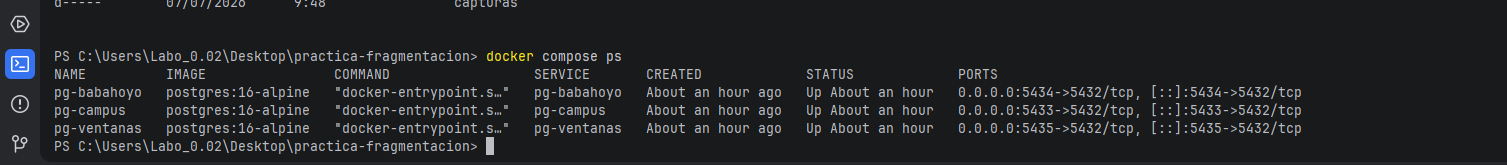
\includegraphics[width=0.9\textwidth]{capturas/docker_ps.png}
}{
\fbox{\parbox{0.85\textwidth}{Insertar captura: docker compose ps mostrando los tres contenedores activos.}}
}
\caption{Contenedores PostgreSQL levantados correctamente.}
\end{figure}

\begin{figure}[H]
\centering
\IfFileExists{capturas/pedidos_global.png}{
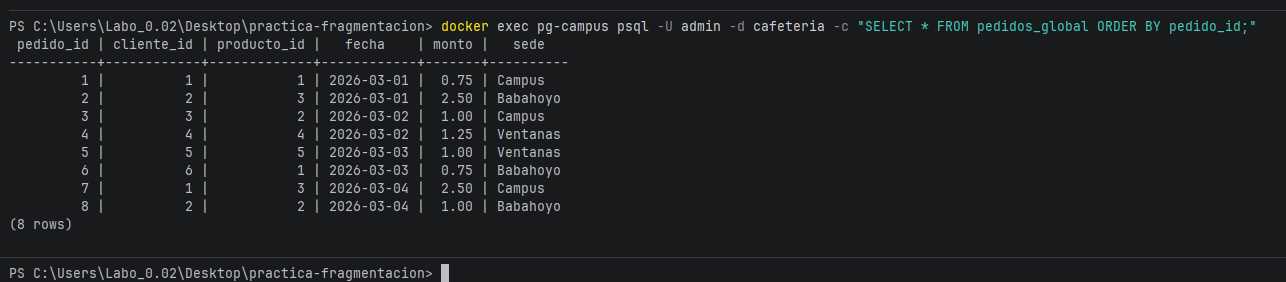
\includegraphics[width=0.9\textwidth]{capturas/pedidos_global.png}
}{
\fbox{\parbox{0.85\textwidth}{Insertar captura: consulta SELECT * FROM pedidos\_global ORDER BY pedido\_id.}}
}
\caption{Reconstrucción global de pedidos.}
\end{figure}

\begin{figure}[H]
\centering
\IfFileExists{capturas/clientes_global.png}{
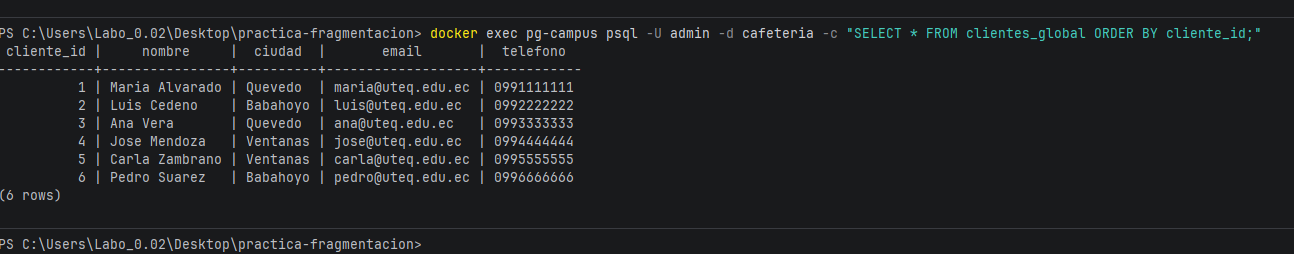
\includegraphics[width=0.9\textwidth]{capturas/clientes_global.png}
}{
\fbox{\parbox{0.85\textwidth}{Insertar captura: consulta SELECT * FROM clientes\_global ORDER BY cliente\_id.}}
}
\caption{Reconstrucción global de clientes.}
\end{figure}

\begin{figure}[H]
\centering
\IfFileExists{capturas/verificacion.png}{
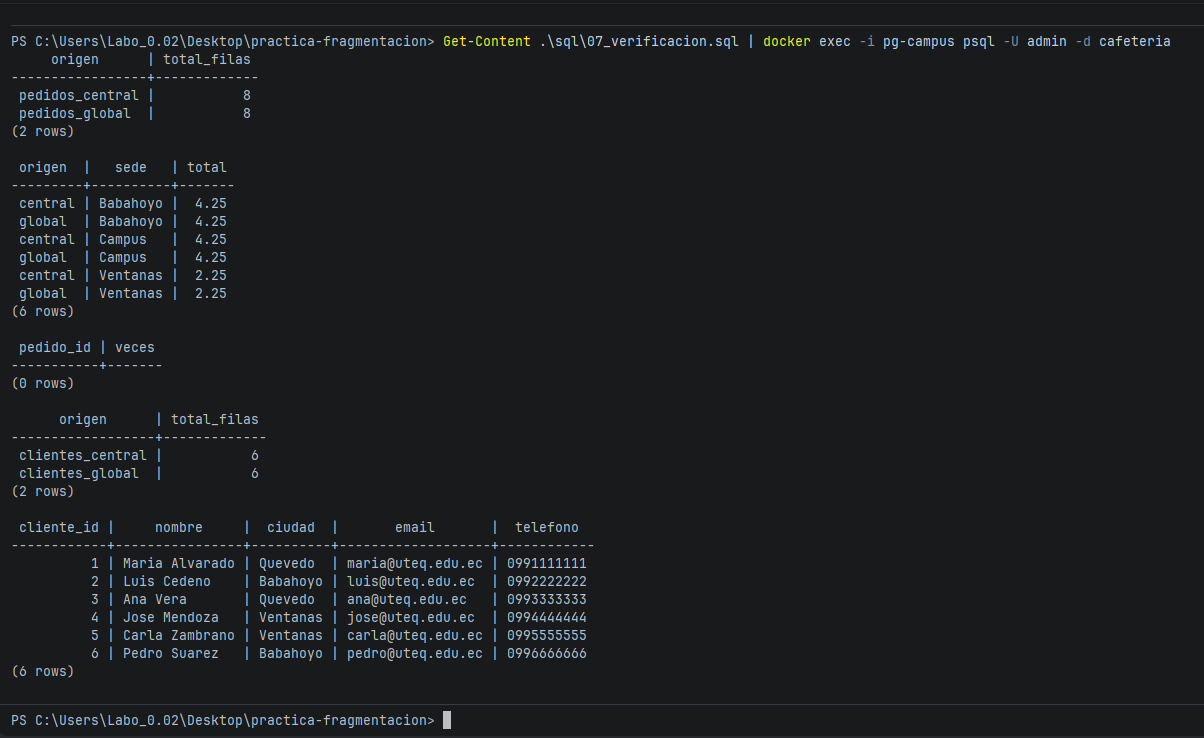
\includegraphics[width=0.9\textwidth]{capturas/verificacion.png}
}{
\fbox{\parbox{0.85\textwidth}{Insertar captura: resultado del script 07\_verificacion.sql.}}
}
\caption{Verificación de completitud, reconstrucción y disjunción.}
\end{figure}

\section{Reflexión}

Durante el desarrollo de la práctica se pudo comprender de manera más clara cómo funciona una base de datos distribuida. Al inicio, la información estaba concentrada en un solo nodo, pero después se dividió en diferentes contenedores, simulando sedes reales de una organización. Esto permitió observar que la fragmentación no consiste solamente en separar datos, sino en hacerlo de forma ordenada y comprobable.

La fragmentación horizontal resultó sencilla de entender porque la tabla \texttt{pedidos} tenía una columna llamada \texttt{sede}. Esta columna permitió enviar cada pedido al nodo correspondiente. En un caso real, esto sería útil porque cada sede podría trabajar principalmente con sus propios datos, reduciendo la carga sobre un servidor central.

La fragmentación vertical permitió observar una ventaja relacionada con la seguridad. Al separar los datos públicos de los datos de contacto, se puede controlar mejor qué usuario o nodo tiene acceso a cierta información. Por ejemplo, un área administrativa podría acceder a correos y teléfonos, mientras que otros usuarios solo verían nombres y ciudades.

La fragmentación mixta fue la parte más compleja porque combina dos criterios al mismo tiempo. Primero se separaron los clientes por ciudad y luego se dividieron sus columnas según el tipo de información. Esta técnica requiere más cuidado porque es fácil olvidar un fragmento o duplicar datos sin darse cuenta.

Una de las principales dificultades fue coordinar correctamente los nodos y los scripts SQL. También fue necesario verificar que cada tabla estuviera en el contenedor correcto. El uso de \texttt{postgres\_fdw} fue importante porque permitió reconstruir los datos desde el nodo Campus, consultando información remota de Babahoyo y Ventanas.

En conclusión, la práctica permitió aplicar conceptos fundamentales de bases de datos distribuidas de forma práctica. Se comprobó que la fragmentación debe cumplir completitud, reconstrucción y disjunción. Además, se entendió que un diseño distribuido puede mejorar la organización y escalabilidad, pero también aumenta la complejidad del sistema.

\section{Preguntas de análisis}

\textbf{1. Si se abre una nueva sede en El Empalme, ¿qué debe cambiar en el diseño horizontal?}

Se debe agregar un nuevo nodo o contenedor para la sede El Empalme y crear un nuevo fragmento horizontal para los pedidos cuya sede sea El Empalme. También habría que actualizar la vista \texttt{pedidos\_global} para incluir el nuevo fragmento mediante otro \texttt{UNION ALL}.

\textbf{2. ¿En qué situaciones la fragmentación vertical mejora la seguridad?}

Mejora la seguridad cuando una tabla contiene datos sensibles que no todos los usuarios deben ver. Por ejemplo, en una tabla de estudiantes se podrían separar los datos públicos, como nombre y carrera, de datos privados como dirección, teléfono o información médica.

\textbf{3. ¿Qué ventaja da que la clave primaria se replique en la fragmentación vertical?}

La clave primaria permite unir nuevamente los fragmentos mediante \texttt{JOIN}. Si no se replicara, no existiría una forma segura de relacionar los datos públicos con los datos privados del mismo registro.

\textbf{4. ¿Por qué la fragmentación horizontal por sede es razonable para pedidos?}

Es razonable porque cada pedido pertenece a una sede específica. De esta manera, cada nodo almacena los pedidos que realmente necesita consultar. Fragmentar por producto no sería tan conveniente porque un mismo producto puede venderse en varias sedes.

\textbf{5. Si se tuviera que soportar tolerancia a fallos, ¿qué se agregaría al diseño?}

Se agregaría replicación de datos. Esto permitiría que si un nodo falla, otro nodo tenga una copia de la información y el sistema pueda seguir funcionando. También sería necesario implementar respaldos automáticos y mecanismos de recuperación.

\section{Conclusiones}

La práctica permitió implementar una base de datos distribuida simulada sobre tres contenedores PostgreSQL. Se aplicó fragmentación horizontal en la tabla \texttt{pedidos}, fragmentación vertical en la tabla \texttt{clientes} y fragmentación mixta combinando criterios de ciudad y sensibilidad de datos.

Los resultados obtenidos demostraron que la fragmentación fue correcta, ya que la vista \texttt{pedidos\_global} devolvió los 8 pedidos originales y la vista \texttt{clientes\_global} reconstruyó los 6 clientes completos. Además, la consulta de disjunción devolvió cero filas, lo que confirmó que no existieron registros duplicados.

Finalmente, se concluye que las bases de datos distribuidas pueden mejorar la organización, seguridad y escalabilidad de un sistema, siempre que el diseño sea cuidadosamente verificado.

\begin{thebibliography}{00}

\bibitem{amer2020ddbs}
A. A. Amer, ``On K-means clustering-based approach for DDBSs design,'' \textit{Journal of Big Data}, vol. 7, no. 31, 2020. doi: 10.1186/s40537-020-00306-9.

\bibitem{ge2021knosys}
Y.-F. Ge, M. Orlowska, J. Cao, H. Wang, and Y. Zhang, ``Knowledge transfer-based distributed differential evolution for dynamic database fragmentation,'' \textit{Knowledge-Based Systems}, vol. 229, art. 107325, 2021. doi: 10.1016/j.knosys.2021.107325.

\bibitem{amer2020heliyon}
A. A. Amer, M. H. Mohamed, and K. Al\_Asri, ``ASGOP: An aggregated similarity-based greedy-oriented approach for relational DDBSs design,'' \textit{Heliyon}, vol. 6, no. 1, art. e03172, 2020. doi: 10.1016/j.heliyon.2020.e03172.

\bibitem{ge2022vldb}
Y.-F. Ge, M. Orlowska, J. Cao, H. Wang, and Y. Zhang, ``MDDE: Multitasking distributed differential evolution for privacy-preserving database fragmentation,'' \textit{The VLDB Journal}, vol. 31, no. 5, pp. 957--975, 2022. doi: 10.1007/s00778-021-00718-w.

\end{thebibliography}

\end{document}
